\subsection{Goals}
We want to answer those questions about our proposed algorithm:
\begin{enumerate}
    \item How fast is it?
    \item How short are the found paths?
\end{enumerate}
Because \textit{fast} and \textit{short} are relative terms. We need to calculate them in a comparison with other approaches. 
We chose to compare our results aginst:
\begin{itemize}
    \item Mikami: known by its speed, but very far from the optimal answer. Would give us insights on how much speed we have achieved.
    \item Steiner Tree: Finds the optimal answer. We will use it to know whether our results are optimal.
    \item Lee Maze: First algorithm used in the industry. Helps us know how far we have progressed relative to the industry practical techniques.
\end{itemize}

\subsection{Code}
We implmented our proposd algorithm in \texttt{mod\_a\_star.py}, 
lee maze algorithm in \texttt{maze\_lee.py},
mikami-tabuchi algorithm in \texttt{mikami\_tabuchi.py}
and steiner tree in \texttt{steiner\_tree.py}.

All scripts read json input from the \texttt{stdin} and writes json output to \texttt{stdout}, so we can chain them with the other scripts. And they follow the \texttt{io\_schema.md} specs about io format.

\subsection{IO Specs}
Input contains a $d\times h \times w$ grid matrix, where:
\begin{itemize}
    \item $d \rightarrow$ Number of layers, either 1 or 2.
    \item $h \rightarrow$ Hieght.
    \item $w \rightarrow$ Width.
\end{itemize}
Each cell is either:
\begin{itemize}
    \item 0 $\rightarrow$ Empty.
    \item 1 $\rightarrow$ Obstacle.
    \item 2 $\rightarrow$ VIA, only when $d=2$ and must exist on the other layer too.
\end{itemize}
Each input contains the source coordinates and a list of targets coordinates.

Output should contain the found paths and their corresponding lengthes.

Both input and output should be in json format. See \texttt{io\_schema.md} for more details.

\subsection{Helper Scripts}
We wrote a couple of scripts to assist with the comparison and testing:
\begin{itemize}
    \item \texttt{gen-input.py}: Generates random input that follows \texttt{io\_schema.md}. It doesn't gurantee that all targets are reachable. For more info \texttt{\$ python3 gen-input.py --help}
    \item \texttt{verify.py}: Takes the input to the algorithm and its output and verifies the correctness of the result. See \texttt{\$ python3 verify.py --help}
    \item \texttt{random\_test}: Generates infinite random inputs, run given algorithm on each test, and verify the results.
    \item \texttt{random\_comp}: Generates $N$ random input, run each algorithm on each input, calls \texttt{calc\_total.py} to calculate total cost and verify the results.
    \item \texttt{nConst}: Calls \texttt{random\_comp} $M$ times, each time with same number of targets, varying the grid area (w,h).
    \item \texttt{areaConst}: Calls \texttt{random\_comp} $M$ times, each time with same width and height of the input grid, varying the number of targets.
    \item \texttt{merge\_comp}: Merges the outputs of \texttt{random\_comp} into one \texttt{tmp/summary.json} with the summary of the experiment.
    \item \texttt{plot.py}: Plots given \texttt{summary.json} through the stdin to \texttt{tmp/plot}.
\end{itemize}

\subsection{The Experiment}
For simplicity, we assumed all grids are squares. So $w=h$ in all tests.
We also assumed number of layers $d=2$ in all tests.

We need to very the area while the number of targets is constant. And in the other case, vary the number of targets while the area is constant.
And in both, we will record and plot the running times and costs.

We expect some algorithm to take a very big time to calculate the output. Unfortunately we can't just let it run forever. So we just sat the timeout as 5 minutes. This is why we collected the number of found targets, so we compare how many times an implmentation has timeouted and resulted in 0 final targets found.

\textbf{Note:} Not all targets in some input have to be reachable. Bigger grids have bigger probability of having non-reachable targets.

We started the experiments by running:
\begin{enumerate}
    \item \texttt{nConst}, which for each area of areas of grid in [10, 15, 20, 50, 100], conducts 5 random experiments on each algo given the same random input (for each experiment) in which the number of targets ($n$) is const and $n = 5$.
    \item \texttt{areaConst}, which for each number of targets in [6, 10, 15, 20, 50], conducts 20 random experiments on each algo given the same random input (for each experiment) in which the area of the grid ($w,h$) is constant and $w = h = 45$.
\end{enumerate}

After running the 2 scripts multiple times and then merging their outputs using \texttt{merge\_comp}, we had so far 396 unique experiment, each experiment is a unique input given to the 4 algorithms and all the 1584 results are in \texttt{summary.json}.

\subsection{Comparisons}
We made the plots using \texttt{plot.py}. The following is the line of thoughts we had through the comparison.

\subsubsection{Running Time Scatter}
We started by scaterring all the running time per \#Targets and per Grid Width, see Fig. (\ref{fig:runningTime}). 

The results are not very clear as the points of mikami and lee are squished down becaus of stein and a*. 

We can also notice a* has some outliers in time, specially in bigger grid widths (50, 100). This is why we may use the median function multiple times instead of the average.

\begin{figure}
\centering

\begin{subfigure}[b]{\linewidth}
    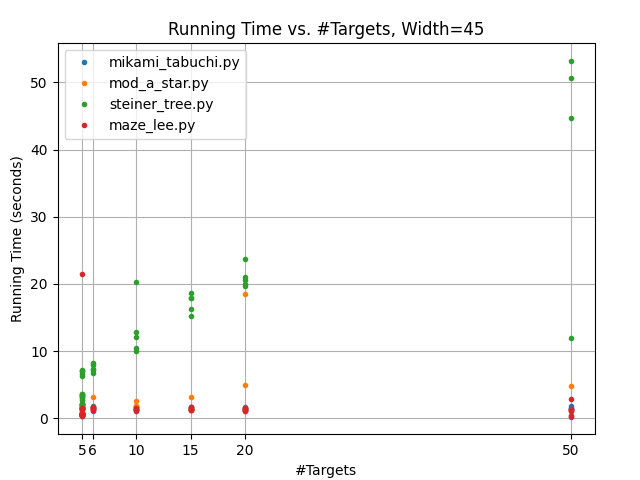
\includegraphics[width=\linewidth]{figures/plots/areaConst.png}
    \caption{Time / \#Targets}
\end{subfigure}
\begin{subfigure}[b]{\linewidth}
    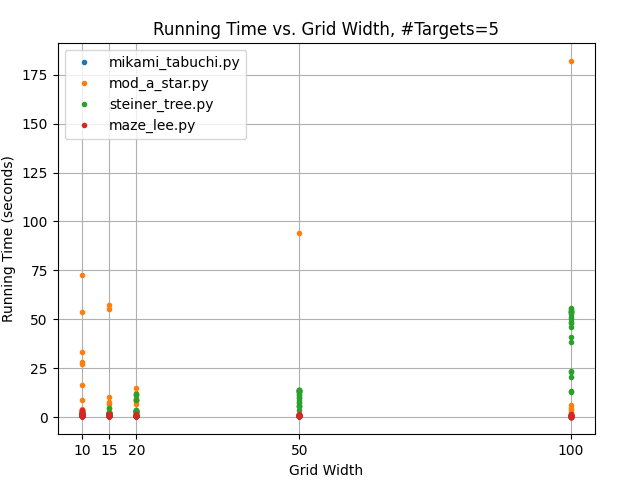
\includegraphics[width=\linewidth]{figures/plots/nConst.png}
    \caption{Time / Grid Width}
\end{subfigure}

\caption{Running Time}
\label{fig:runningTime}
\end{figure}